% -----------------------------------------------------------------------------
% Roteiro de funcionamento
% -----------------------------------------------------------------------------

\chapter{Roteiro de funcionamento}
\label{chap:Roteiro}
Com o objetivo principal de figurar uma ferramenta educacional, o acesso aos dados, o reconhecimento das etapas de funcionamento e troca de mensagens entre as camadas foram os principais focos do desenvolvimento. Tendo em mente tal premissa a execução da ferramenta segue exatamente as mesmas etapas da troca de mensagens que ocorre no modelo de protocolos TCP/IP.

A execuç\~ao \'e iniciada com uma requisiç\~ao http feita a partir de um browser, a camada responsável pela Aplicação recebe essa mensagem faz o reconhecimento de seu conteúdo e repassa para camada seguinte de Transporte. Os dados da referentes a uma requisição HTTP incluem o método, identificação do cliente, versão http, o host para o qual está se fazendo a requisição e características do cliente.

%ponho ou não??
Os principais métodos de requisição HTTP são apresentado, sucintamente na Tabela \ref{tab:requisicoesHTTP}, e como exemplo segue uma solicitação gerada em testes a qual é apresentada ao usuário.

\begin{table}[H]
	\centering
	\small
	\begin{tabular}{ |p{2cm}||p{7cm}| }
		\hline
		Método & Descrição\\
		\hline 
		GET   	& Lê uma pagina Web\\
		HEAD	& Lê um cabeçalho de página Web\\
		POST 	& Acrescenta algo a uma página Web\\
		PUT    	& Armazena uma página Web\\
		DELETE	& Remove a página Web\\
		TRACE	& Ecoa a solicitação recebida\\
		CONNECT & Conecta através de um proxy\\
		OPTIONS & Consulta opções para uma página\\
		\hline
	\end{tabular}
	\caption {Métodos de requisição HTTP}
	\label {tab:requisicoesHTTP}
	\cite{TANENBAUM}
\end{table}

\noindent
GET /test.html HTTP/1.1\\
Host: localhost:1111\\
Connection: keep-alive\\
Upgrade-Insecure-Requests: 1\\
User-Agent: Mozilla/5.0 (X11; Linux x86\_64) AppleWebKit/537.36 (KHTML, like Gecko)
Chrome/54.0.2840.71 Safari/537.36\\
Accept: text/html,application/xhtml+xml,application/xml;q=0.9,image/webp,*/*;q=0.8\\
Accept-Encoding: gzip, deflate, sdch, br\\
Accept-Language: en-US,en;q=0.8,pt;q=0.6,pt-BR;q=0.4\\

Ao receber o pacote de requisição da camada superior, na camada de Transporte o usuário tem a opção entre dois tipos de protocolos o UDP e o TCP. Caso a escolha do usuário seja UDP \'e adicionado ao seguimento apenas a porta de origem e destino, o comprimento do UDP, incluindo cabeçalho e o \textit{checksum} para verificação.

Caso a escolha do usuário seja utilizar o protocolo de transporte TCP, além dos dados reunidos pelo protocolo UDP, é adicionado ao cabeçalho o número de sequência, o número de confirmação, o tamanho da janela, ponteiro para urgente, opções e as flags. Ao todo são oito \textit{flags}: 

\begin{itemize}
	\item CWR e ECE: utilizadas para sinalizar congestionamento.
	\item URG: indicador para o caso de uso do ponteiro de urgência.
	\item ACK: verifica se o número de confirmação é válido.
	\item PSH: declara o modo \textit{push} solicitando ao que o receptor a entregar os dados à aplicação ao invés de armazena-los até que um \textit{buffer} completo tenha sido recebido.
	\item RST: utilizado para reiniciar uma conexão.
	\item SYN: usado para estabelecer conex\~oes
	\item FIN: encerra uma conex\~ao
\end{itemize}

Duas dessas flags s\~ao de especial import\^ancia pois s\~ao respons\'aveis pelo estabelecimento da conex\~ao entre o cliente e o servidor, o que garante a confiabilidade da conversaç\~ao. As flags SYN e ACK s\~ao utilizadas pelo procedimento conhecido como \textit{Tree Way Handshake}, representado na Figura \ref{fig:3wh}.

\begin{figure}
	\centering
	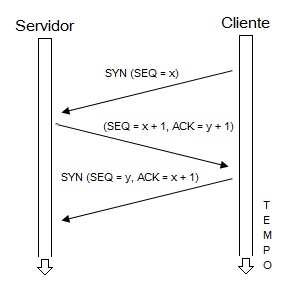
\includegraphics{04-figuras/3wh.png}
	\caption{Three Way Handshake - Estabelecimento de conexão TCP}
	\cite{TANENBAUM}
	\label{fig:3wh}
\end{figure}

Quando um cliente deseja estabelecer  com  um servidor, este envia um seguimento com a flag SYN igual a 1, o que ser\'a reconhecido pelo servidor como um pedido para o estabelecimento de uma conex\~ao e se o cliente receber um seguimento como resposta contendo as flags SYN e ACK iguais a 1 indica que a requisiç\~ao foi aceita pelo servidor. O cliente envia, ent\~ao, por \'ultimo um seguimento com a flag ACK igual a 1, indicando o reconhecimento da resposta.

Em ambos os casos as PDU's são apresentadas ao usuário e, no caso do protocolo TCP, s passos realizados pelo \textit{three way handshake} também são reportados ao serem executados. 

\begin{figure}[H]
	\centering
	\subfloat[Protocolo UDP]{
		\label{subfig-1:transOutput}
		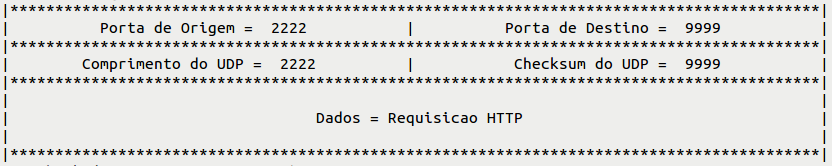
\includegraphics[width=\textwidth] {04-figuras/ssUDP.png}
	} \\
	\subfloat[Protocolo TCP]{
		\label{subfig-2:transOutput}
		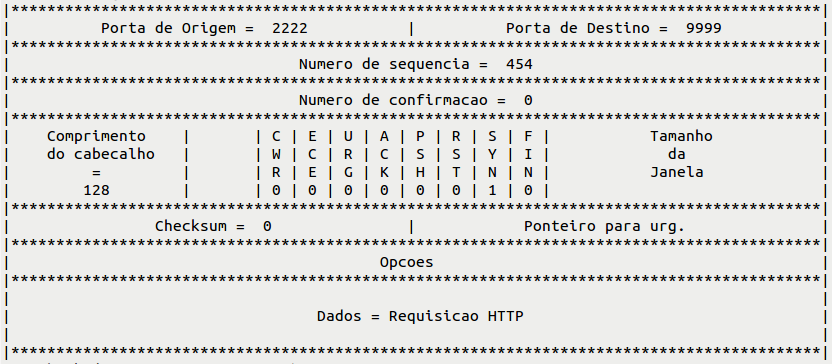
\includegraphics[width=\textwidth] {04-figuras/ssTCP.png}
	}
	\caption{Resultados obtidos na execução do módulo de simulação referente a camada de Transporte}
	\label{fig:transOutput}
\end{figure}